\begin{center}\large\textbf{Readings: 17.6}\\
\normalsize \end{center}
\large ~\hrulefill
~\\
So far, we have considered complete factorial experiments.  That is, experiments where the responses were measured at every possible combination of levels of the experimental factors.  \\~\\
Now we will consider factors that are \textit{nested}.  That is, in which responses are measured at a subset of the combination of factor levels.  \\~\\
\textbf{Crossed vs Nested factors}\\~\\
\textbf{Crossed} - The levels of factor A are said to be \textit{crossed} with the levels of factor B if every level of A occurs in combination with every level of B.\\~\\
\textbf{Nested} - Factor $B$ is \textit{nested} in factor $A$ if the levels of factor $B$ differ for at least one level of factor $A$.\\~\\

\newpage

\textbf{A Nested Design Example:}\\
Experiment to study effect of drug and method of administration on fasting blood sugar in diabetic patients
\begin{itemize}
\item First factor is drug: brand I tablet, brand II tablet, insulin injection 
\item Second factor is type of administration (see table)
\end{itemize}

\begin{center}
\begin{tabular}{|llccc|} \hline
Drug & Type of & Mean & Variance & Mean (Grand mean = $\bar{y}_{\bullet\bullet\bullet}=22.3$).\\
($i$) & Administration $(j)$ & $\bar{y}_{(i)j}$ & $s_{(i)j}^2$ & $\bar{y}_{(i)\bullet}$\\ \hline
Brand I tablet & $30 mg \times 1$ & 15.7 & 6.3 & 17.7\\
& $15 mg \times 2$ & 19.7 & 9.3 & \\
Brand II tablet & $20 mg \times 1$ & 20 & 1 & 18.7 \\
& $10 mg \times 2$ & 17.3 & 6.3 & \\
Insulin injection & before breakfast  & 28  & 4 & 30.5\\
& before supper & 33 & 9 & \\ \hline
\end{tabular}
\end{center}
~\\~\\~\\~\\~\\
\textcolor{red}{We use the notation B(A) for factor B nested in factor A, and we use $b_{(i)j}$ to say level $j$ of factor B for the $i^{th}$ level of factor A.  \\~\\
Here, factor B is administration and factor A is Drug.  We would say administration is nested in drug or B(A).  \\~\\
The level of factor B, `before supper', would be labeled $b_{(3)2}$ and `10 mg x 2' would be $b_{(2)2}$.\\~\\}

\newpage

In the following examples identify which pairs of factors are crossed and which are nested.
\begin{itemize}
\item The amount of vitamin A in jars of baby food might vary from brand to brand and might also vary between flavors of the same brand. To study the effect of these two factors on vitamin A content, a researcher randomly selected the three major brands of baby food in the area.\\
For Brand 1 they selected carrot and pear, for Brand 2 sweet potato and green bean, and for Brand 3 pea and squash.   Five jars were selected for each treatment.\\~\\%~\\~\\~\\
\textcolor{red}{Factors are Brand and Flavor.  Brand has 3 levels, flavor has 2 levels and the levels depend on Brand, so flavor is nested in brand.  Flavor(Brand).}\\~\\
\item Gum arabic is used to lengthen the shelf life of emulsions. It comes from acacia trees and is processed for use in emulsions. Eight raw gum arabic samples are obtained from each of two different varieties of acacia tree (for a total of sixteen samples.)  Four samples from each variety of acacia tree are randomly assigned an experimental treatment (the others act as a control).  The sixteen samples are dried, and an emulsion made from each. The response is the time until the emulsion begins to separate.\\~\\%~\\~\\~\\
\textcolor{red}{Factors are Variety and Treatment.  Variety has 2 levels, treatment has 2 levels (trt or control).  These are all observed together so this is a crossed experiment.}\\
\item A total of 30 participants each read a story and were asked to recall some facts from the story. The dependent variable was number of facts recalled. There were two variables of interest.  One was the story setting (stories were either familiar or exotic).  For each type of story setting there were three different stories (for a total of 6 totally different stories).  Each story was read by 5 people and the number of facts recalled were recorded.\\~\\
\textcolor{red}{Factors are setting and story.  Setting has 2 levels and Story has 3 levels.  The levels of the story depend on the setting so story is nested in setting.  Story(Setting).\\~\\
Note: Story would probably be considered random.  More on this later.}
\end{itemize}

\newpage

Again, we use the notation B(A) for factor B nested in factor A, and we use $b_{(i)j}$ to say level $j$ of factor B for the $i^{th}$ level of factor A.  The model for analysis of a two-factor nested design is:
$$Y_{ijk}=\mu+\tau_i+\beta_{(i)j}+E_{ijk},~~E_{ijk}\sim^{iid} N(0,\sigma^2)$$
$$i=1,2,\ldots,a ~~~j=1,2,\ldots,b_{i} ~~~k=1,2,\ldots,n_{ij}~~~\mbox{with some sum to zero constraints}$$
What are the interpretations of each parameter in the above model?
\begin{itemize}
\item $\mu$ - \textcolor{red}{overall mean}
\item $\tau_i$ - \textcolor{red}{effect of level i of factor A}
\item $\beta_{(i)j}$ - \textcolor{red}{effect of level j of B for level i of A}\\
\end{itemize}
A partial ANOVA table (with expected mean squares) for a nested design is given below, fill it in\\
\begin{tabular}{l|lllll}
source& df &SS & MS & EMS & F\\
\hline
&&&&&\\
A & $a-1$ & SS(A) & $MS(A)=%~~~~~~~~~~~~~~~~~~~
\textcolor{red}{\frac{SS(A)}{a-1}}
$&$\sigma^2+nb\psi^2_A$& F=
$\textcolor{red}{\frac{MS(A)}{MS(E)}}$
\\
&&&&&\\
B(A) & $\sum_{i=1}^{a}b_{i}-a$ & SS(B(A)) & $MS(B(A))=%~~~~~~~~~~~~~~~~
\textcolor{red}{\frac{SS(B(A))}{\sum_{i=1}^{a}b_{i}-a}}
$&$\sigma^2+n\psi^2_{B(A)}$&F=
$\textcolor{red}{\frac{MS(B(A))}{MS(E)}}$
\\
&&&&&\\
Error & $N-\sum_{i=1}^{a}b_i$& SS(E)& $MS(E)=%~~~~~~~~~~~~~~~~~~~
\textcolor{red}{\frac{SS(E)}{N-\sum_{i=1}^{a}b_i}}
$&$\sigma^2$\\~\\
\end{tabular}\\
The null and alternative hypotheses of interest for a nested experiment are 
$$\mbox{Global test~~} H_0:\tau_i=0 \mbox{ for all i and }\beta_{(i)j}=0\mbox{ for all i, j     }H_A: \mbox{At least 1 differs}$$
$$\mbox{Test for effect of A } H_0:\tau_i=0 \mbox{ for all i   } H_A: \mbox{At least 1 differs}$$
$$\mbox{Test for nested factor B }H_0:\beta_{(i)j}=0\mbox{ for all i, j     } H_A: \mbox{At least 1 differs}$$
and these hypotheses jointly (the global test).  In words, what are each of these hypotheses testing?\\~\\%~\\~\\~\\~\\~\\
\textcolor{red}{Global: Is anything in the model useful?\\
$\tau_i$ all 0: does factor A have an effect?\\
$\beta_{(i)j}=0$ for all i,j: do any of the levels of factor B differ from each other?}\\~\\
Assuming the above null hypotheses are true, what value is expected for each F in the above ANOVA table?  What values give evidence against these
$H_0$'s?\\~\\%~\\~\\~\\
\textcolor{red}{F's should be approximately 1 under $H_0$.  F's larger than 1 give evidence for $H_A$.}
\\

There is no interaction being tested here, why do you think that is not something we look at for a nested design?
\textcolor{red}{Can't inspect interaction!  No level of B at each level of A!}

\newpage

\noindent Another Example: The amount of readily soluble phosphorus in a large number of soil samples was to be determined in a lab that employed six technicians.  \textbf{Three worked in the morning and three at night.}  To determine whether the measured values of phosphorus (lb/acre) were affected by the time of day (am or pm) and the technician making the measurement, 24 identical specimen samples were assigned to the six technicians at random (each got 4 samples).  They analyzed the samples and the data was recorded. \\
\begin{center}
\begin{tabular}{cc|c|c}
Time & Technician & Response & Mean $\bar{y}_{(i)j}$\\\hline
AM & 1 &42,44,43,44 & $\bar{y}_{(1)1}=43.25$\\
AM & 2&43,44,45,42& $\bar{y}_{(1)2}=43.50$\\
AM &3&47,46,47,43& $\bar{y}_{(1)3}=45.75$\\
PM &1&50,49,52,50& $\bar{y}_{(2)1}=50.25$\\
PM &2&49,48,49,47& $\bar{y}_{(2)2}=48.25$\\
PM &3&47,51,46,48& $\bar{y}_{(2)3}=48.00$\\
\end{tabular}	
~\\Note: Technician 1 in the AM is different than technician 1 in the PM.
\end{center}

What are the factors in this study?  Which factor is nested in the other?\\~\\%~\\~\\~\\~\\~\\~\\
\textcolor{red}{Time, Technician.  Technician(Time)}\\~\\~\\~\\~\\
(Let's consider technician as fixed for now.)  Write out the statistical model for these data and interpret $\mu$, $\tau_i$ and $\beta_{(i)j}$ in terms of the experiment.\\~\\
\textcolor{red}{$$Y_{ijk}=\mu+\tau_i+\beta_{(i)j}+E_{ijk}~~~~~~E_{ijk}\sim^{iid}N(0,\sigma^2)$$
$$\mu= \mbox{ overall mean amount of readily soluble phosphorus}$$
$$\tau_i = \mbox{ effect of time (AM=1 or PM=2)}$$
$$\beta_{(i)j}= \mbox{ effect of technician j at time i}$$
}

\newpage

The model is fit in SAS using the code here:\\
\begin{small}
\begin{verbatim}
proc glm data=phosph;
class time technician;
model y=time technician(time);
run;
\end{verbatim}
\end{small}

\begin{center}
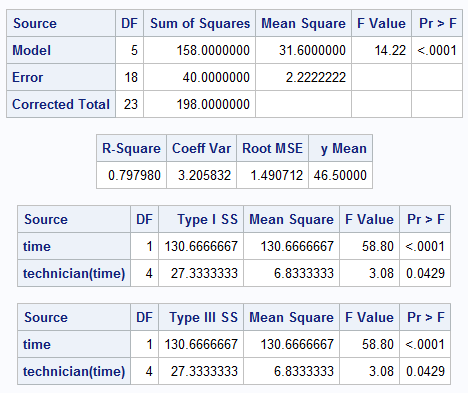
\includegraphics[scale=0.65]{NestedSAS1}\\
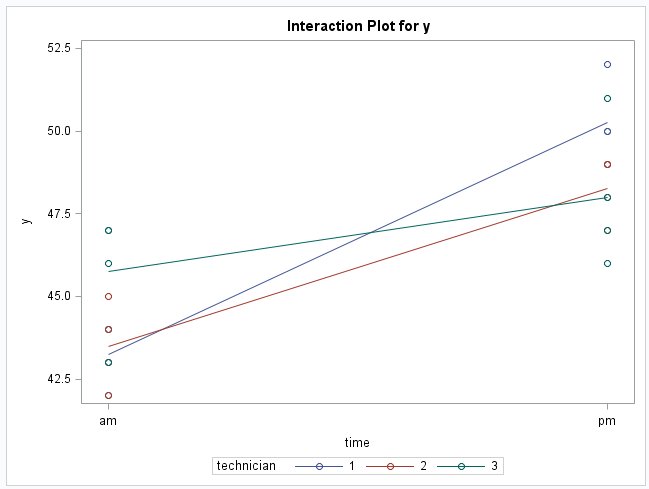
\includegraphics[scale=0.4]{NestedSAS2}
\end{center}
\begin{enumerate}
\item The first step is to check that anything in our model is useful.  Which p-value tests this? What is the null hypothesis?\\~\\%~\\~\\~\\
\textcolor{red}{The global test in the ANOVA table tests this hypothesis.  P-value$<$0.0001 so reject $H_0:\tau_i\mbox{ all 0 and }\beta_{(i)j} \mbox{ all 0}$ in favor of $H_A:$ at least one of those parameters is not 0.}
\newpage

\item The next step in the analysis is to test the significance of the difference between technicians.  Which p-value tests this?  What is the null hypothesis?  Interpret your conclusions.\\~\\%~\\~\\~\\
\textcolor{red}{p-value=0.0429 $<$0.05, Reject $H_0: \beta_{(i)j}$ all 0 in favor of $H_A$ that at least one is not 0.  \\
Conclusion: Technicians vary in at least one of the times.}\\~\\

\item We also want to inspect the difference between am and pm.  Which p-value tests this?  What is the null hypothesis?  Interpret your conclusions.\\~\\%~\\~\\~\\~\\~\\
\textcolor{red}{p-value$<0.0001<$0.05, Reject $H_0: \tau_{i}$ all 0 in favor of $H_A$ that at least one is not 0.  \\
Conclusion: Time has an effect on the response.}\\~\\

\item Is the interaction plot given by SAS meaningful?  Why?\\~\\%~\\~\\~\\~\\
\textcolor{red}{No, technician 1 in the AM doesn't have any relationship with technician 1 in the PM.  The labels are arbitrary so the connected lines are not meaningful.}\\~\\

\item Since both are significant, we want to compare the difference between technicians at a given time, then also compare the two time levels.  \\~\\
These can be inspected by adding the following SAS command:\\
\begin{small}
\begin{verbatim}
proc glm data=phosph plots=NONE; class time technician;
model y=time technician(time)/clparm;
lsmeans time technician(time)/adjust=tukey cl;
estimate 'effect of Time' intercept 0 time 3 -3 technician(time) 1 1 1 -1 -1 -1/divisor=3; 
estimate 'effect of Tech 1/2 within Time=AM' intercept 0 time 0 0 technician(time) 1 -1 0 0 0 0;
estimate 'effect of Tech 1/3 within Time=AM' intercept 0 time 0 0 technician(time) 1 0 -1 0 0 0;
estimate 'effect of Tech 2/3 within Time=AM' intercept 0 time 0 0 technician(time) 0 1 -1  0 0 0;
estimate 'effect of Tech 1/2 within Time=PM' intercept 0 time 0 0 technician(time) 0 0 0 1 -1 0;
estimate 'effect of Tech 1/3 within Time=PM' intercept 0 time 0 0 technician(time) 0 0 0 1 0 -1;
estimate 'effect of Tech 2/3 within Time=PM' intercept 0 time 0 0 technician(time) 0 0 0 0 1 -1; run;
\end{verbatim}
\end{small}

\newpage

Output from estimate statements (note, these CI's are not corrected for Multiple comparisons!)

\begin{center}
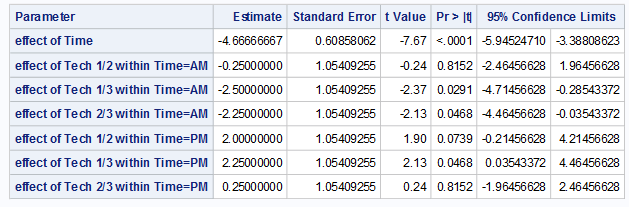
\includegraphics[scale=0.7]{NestedSAS5}
\end{center}


Output from lsmeans statements (note, we probably don't care about all of the differences between technicians!)

\begin{center}
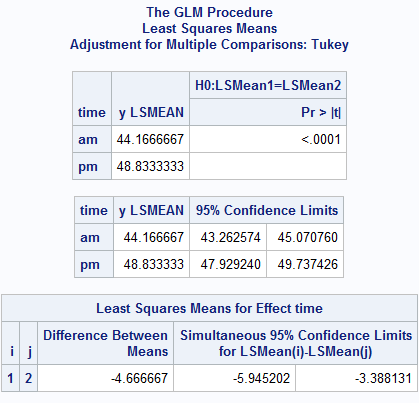
\includegraphics[scale=0.7]{NestedSAS3}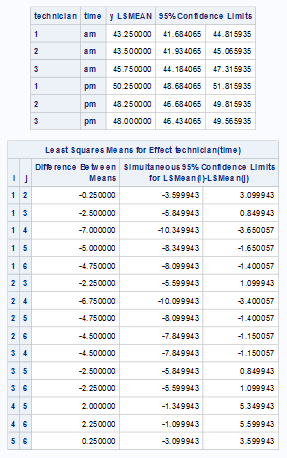
\includegraphics[scale=1]{NestedSAS4}
\end{center}

\end{enumerate}